\documentclass[10pt]{article}         %% What type of document you're writing.

%%%%% Preamble

%% Packages to use

\usepackage{amsmath,amsfonts,amssymb,url}   %% AMS mathematics macros
\usepackage[numbers,sort&compress]{natbib}
\usepackage{graphicx}
\usepackage{subcaption}
\usepackage[svgnames]{xcolor}
\usepackage{listings}


\graphicspath{ {./images/} }
%% Title Information.

\lstset{language=R,
    basicstyle=\small\ttfamily,
    stringstyle=\color{DarkGreen},
    otherkeywords={0,1,2,3,4,5,6,7,8,9},
    morekeywords={TRUE,FALSE},
    deletekeywords={data,frame,length,as,character},
    keywordstyle=\color{blue},
    commentstyle=\color{DarkGreen},
}

\title{SI model with enviromental transmission}
\author{Petr Kouba}
%% \date{1 July 2004}           %% By default, LaTeX uses the current date

%%%%% The Document

\begin{document}
\maketitle

\section{Continuous model - PDEs}
\label{continuous}
I tried to write down the model in the continuous case by myself, I was not sure how to write down the relation of aging and the flow of time efficiently so I searched for this and found the nice way of just adding the partial derivatives with respect to age and time, as in the Von Foerster - McKendrick equation\cite{McKendrick}:

\begin{equation}
	\frac{\partial D(a,t)}{\partial t} + \frac{\partial D(a,t)}{\partial a}= \Lambda(a,t) - f(a)D(a,t)P(t) - \delta^{sus}(a)D(a,t)
\end{equation}

\begin{equation}
	\frac{\partial I(a,t)}{\partial t} + \frac{\partial I(a,t)}{\partial a}= f(a)D(a,t)P(t) - \delta^{inf}(a)I(a,t)
\end{equation}

\begin{equation}
	\frac{\partial P(t)}{\partial t}= \int_{0}^{\inf} \delta(a)^{inf} I(a,t)b \, da - \delta^{pat}P(t)
\end{equation} \newline
\newline
\textbf{Initial conditions:}  \newline
$D(a,0)=\Psi(a)$ ... initial age distribution of susceptibles \newline
$I(a,0)=\Phi(a)$ ... initial age distribution of infecteds \newline
$P(0)$ ... initial number of parasytes in the environment \newline
\newline
\textbf{Definition of variables:}  \newline
$D(a,t)$ 	...		number of susceptible Daphnias of age a, in time t	\newline
$I(a,t)$ 	...		number of infected Daphnias of age a, in time t \newline
$P(t)$	...		number of pathogens in the environment, which can infect \newline
Newborns ($r(a)$ is an age dependant reproductive rate):
\[
    \Lambda(a,t)= 
\begin{cases}
    \int_0^{\inf}r(a)D(a,t)\, da,& \text{if } a = 0\\
    0,              & \text{otherwise}
\end{cases}
\]
$f(a)$ ... age dependent susceptibility \newline
$\delta(a)^{sus}$ ... age dependent death rate of susceptible individuals \newline\newline
$\delta(a)^{inf} = \delta(a)^{sus} + v(a)$ ... age dependent death rate of infected individuals, obtained by summing the death rate of susceptibles and age dependent virulence \newline
$\delta^{pat}$ ... constant death rate of pathogens in the environment \newline
$b$ ... number of new pathogens released to the environment after death of an infected infividual\newline
\newline
\textbf{Assumptions:}

\begin{enumerate}
\item The above model does not reflect the carrying capacity of the environment, it could be reflected by considering death and birth rates depending on the total population size (population density), through which the death and reproductive rates could implicitely also obtain time dependence. (?) But in our discrete model this will be taken care of by the normalization to carrying capacity
\item We neglect the age structure of the pathogens in the environment and therefore (together with the above assumption) consider their death rate to be constant
\item Infected individuals are sterilized immediately and therefore are not giveng birth to new offsprings and new offsrings cannot be born with inhereted pathogen (therefore births are only in favor of the compartment of suceptibles)
\item The infectiousnes of a burst $b$ is constant (But actually it might be correlated with the duration of infection, so that would be possible improvement in the model)
\end{enumerate}
\newpage
\section{Current model as implemented in the sample R file "age-model.Rmd"}
\label{rcode}
\textbf{The relevant part of the code (performing the time evolution):}
\begin{lstlisting}
    for(t in 1:t.end){
        ## let fleas reproduce:
        newborns <- sum(r*D)
        ## dying:
        D <- (1-m)*D
        ## age every flea:
        D.new <- c(newborns,D[-length(D)])

        ## dying by infection:
        I <- (1-v)*I
        P <- sum(v*I)
        ## new infections:
        I.new <- b*P*f*D
        ## age every flea:
        I <- I.new + c(0,I[-length(I)])
        
        ## shrink to carrying capacity:
        D <- D.new
        if(sum(I)+sum(D) > K){
            D <- D * K/(sum(I)+sum(D))
            I <- I * K/(sum(I)+sum(D))
        }
        output <- rbind(output,
                        c(t,P,D,I))
    }
    output
}

\end{lstlisting}
\newpage
\textbf{Differences with respect to Section~\ref{continuous} and suggestions to make both models compatible}

\begin{itemize}
	\item The model is of course discretized, which comes with further assumptions: giving birth, dying and getting infected takes exactly one time step
	\item Normalization to carrying capacity is implemented
	\item Death of infecteds is only due to infection, perhaps there should be:\newline $I \leftarrow (1-v-m)I$ istead of $I \leftarrow (1-v)I$
	\item Pathogens are assumed to be alive exactly one time step, is this on purpose? If not, their dynamics should be as following (to reflect both their actual death rate as well as incrementing the populatin with each birth, instead of overwriting): \newline
	$ P \leftarrow (1-\delta^{pat})*(P + sum((v+m)*I))$
	\item The only mechanism causing the loss of susceptibles is due to death, loss of susceptibles due to becoming infected was probably forgotten in the model. $ D \leftarrow (1-m)*D$ should be replaced by $ D \leftarrow (1-m-b*f*P)*D$
\end{itemize}
\newpage
\section{Model of survival used for estimation of delta based on the experimental data}

In the model, which we used for the estimation of delta in control population, exposed population and in the infected population, we had the following assumptions:\newline
\newline
\textbf{Assumptions}
\begin{enumerate}
	\item No births
	\item No interaction between the control, infected and exposed population
\end{enumerate}

\begin{figure}[h]
\begin{subfigure}[b]{0.5\textwidth}
    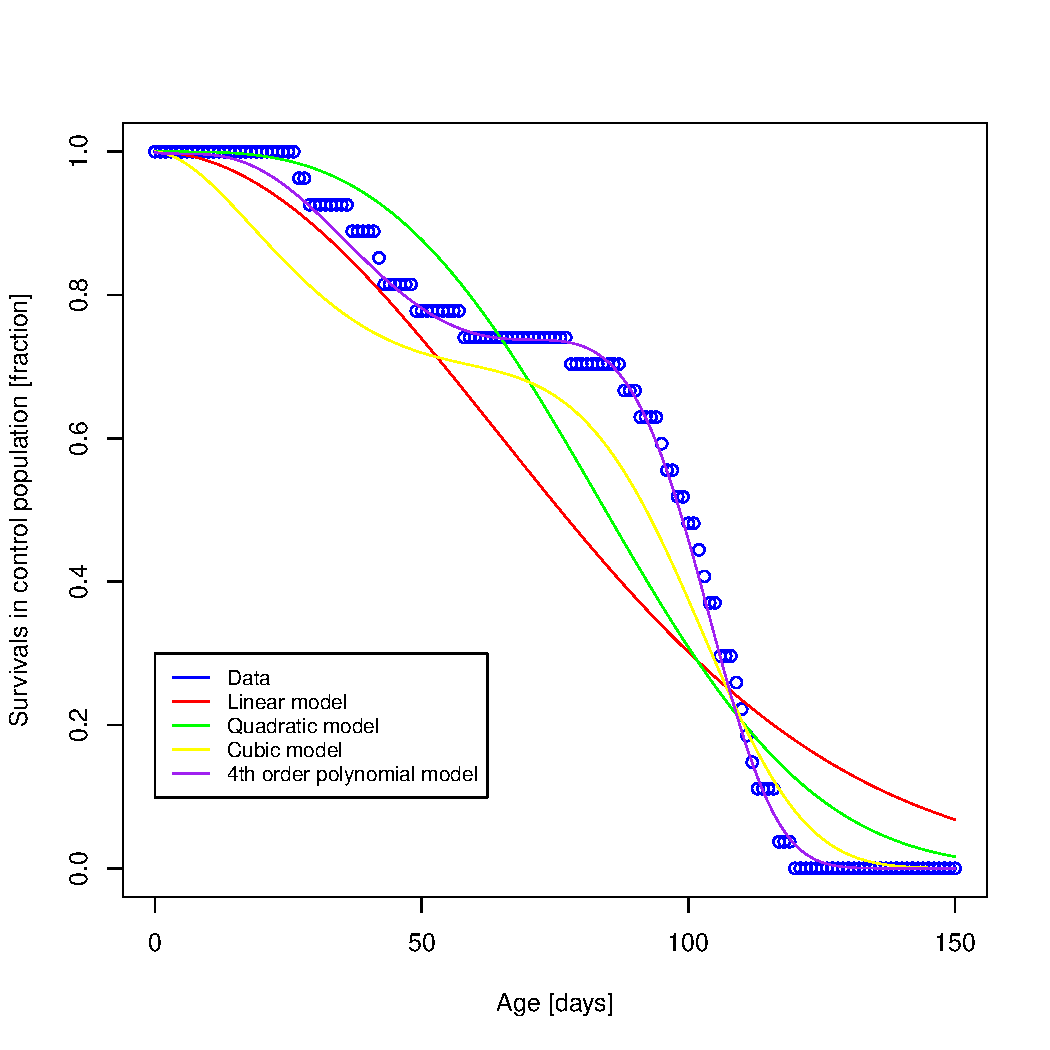
\includegraphics[width=\textwidth]{Control_population_survival.pdf}
    \caption{Survival of the control population}
    \label{fig:subfigure_1}
  \end{subfigure}
  %
  \begin{subfigure}[b]{0.5\textwidth}
    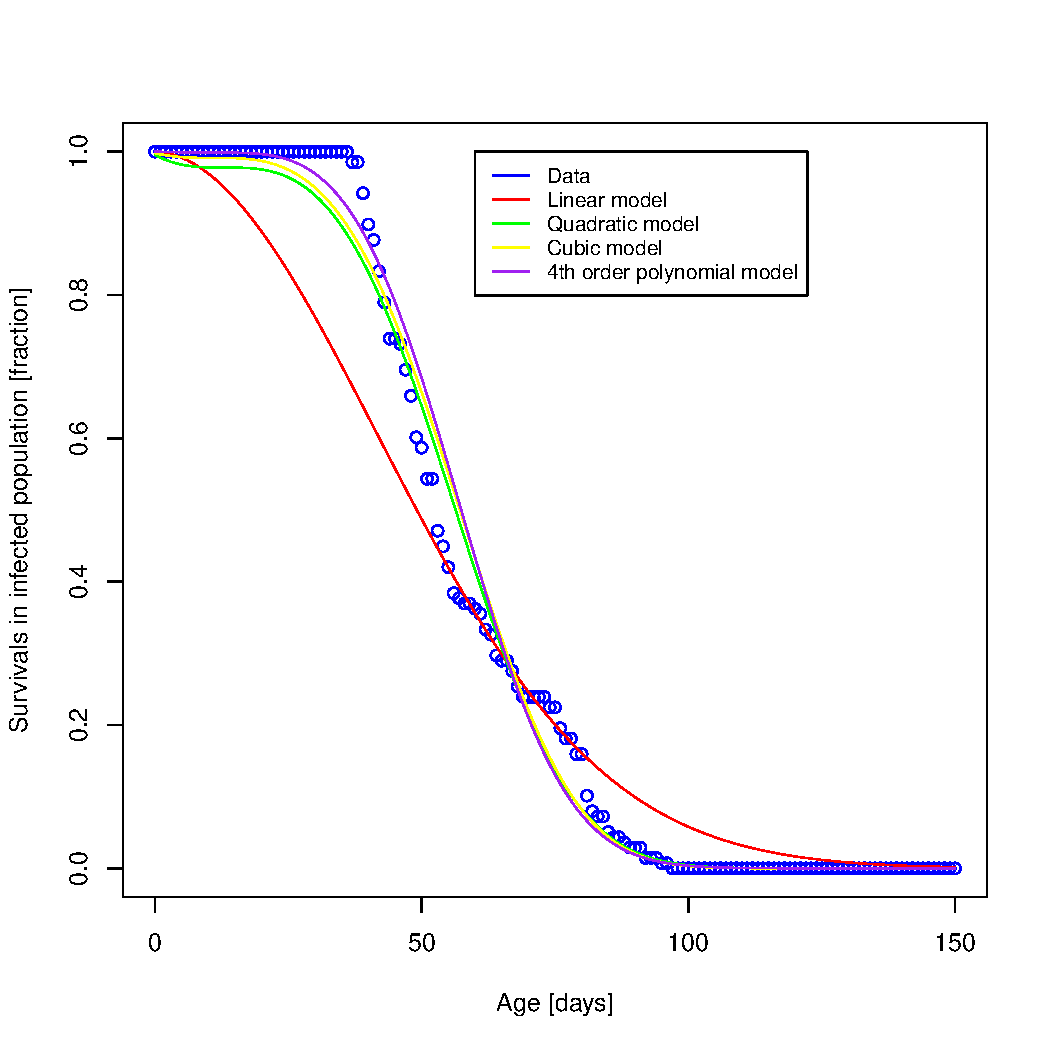
\includegraphics[width=\textwidth]{Infected_population_survival.pdf}
    \caption{Survival of the infected population}
    \label{fig:subfigure_2}
  \end{subfigure}
\caption{Plots of survivals used for the MLE of delta}
	\label{fig:survival_curve}
\end{figure}

From these assumptions it follows that the only mechanisms left in the time evolution were aging and dying (both dying due to aging and dying due to infection). We simply took the initial number of infecteds and susceptibles, considered their age to be 0 and let them evolve separately only under the process of dying.This model produced the survival plots in Figure ~\ref{fig:survival_curve}.

We can use the model described in Section~\ref{rcode} to reproduce the plots in the Figure~\ref{fig:survival_curve} be picking very specific cases. 

To obtain the plot in Figure~\ref{fig:subfigure_1} using our model from Section ~\ref{rcode}, we set the vector of the age dependent reproduction r[] to a null vector and for mortality m[] we pick the delta obtained from the 4th order polynomial Ansatz during our MLE optimization. Since the plot in the Figure~\ref{fig:subfigure_1} is 2D and corresponds to the projection $D(a,t)=D(a,t=a)$ we will also restrict our plot, which could in principle be 3D (age and time could generally be independent variables), to this projection. We can compare the the obtained plots in the Figure ~\ref{fig:subfigure_3}. 

To obtain the plot in Figure~\ref{fig:subfigure_2} using our model from Section ~\ref{rcode}, we set either $b=0$ or f[] to a null vector to decouple the infected population from the susceptibles. Further, we use the delta obtained from the 2nd order polynomial Ansatz for MLE fitting of the data for the infected population as our overall death rate of the infecteds (v[]+m[]). We again plot the projection of the survival along the axis $t=a$. We can compare the the obtained plots in the Figure~\ref{fig:subfigure_4}. 

\begin{figure}[h]
\begin{subfigure}[b]{0.5\textwidth}
    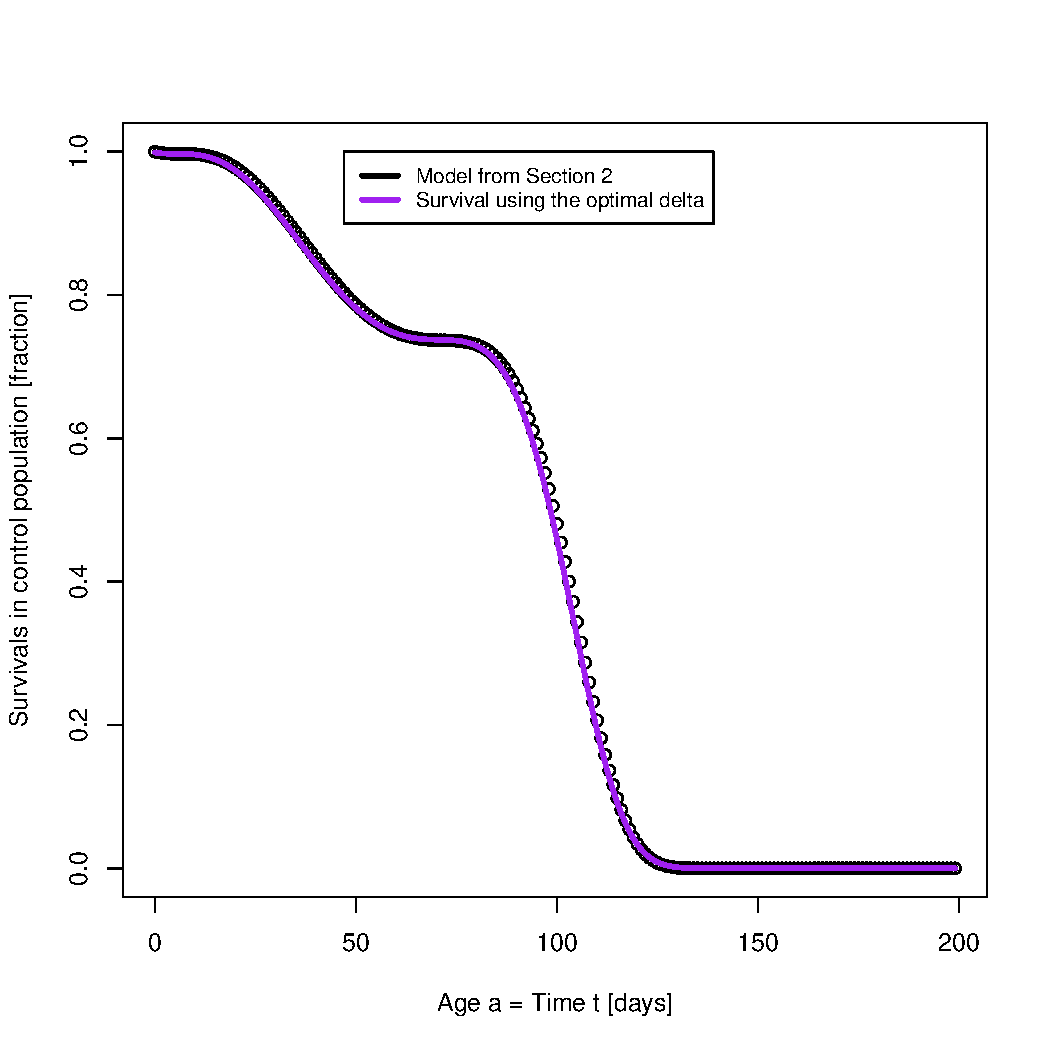
\includegraphics[width=\textwidth]{Comparison_of_models_control.pdf}
    \caption{Comparison of the models for the control population}
    \label{fig:subfigure_3}
  \end{subfigure}
  %
  \begin{subfigure}[b]{0.5\textwidth}
    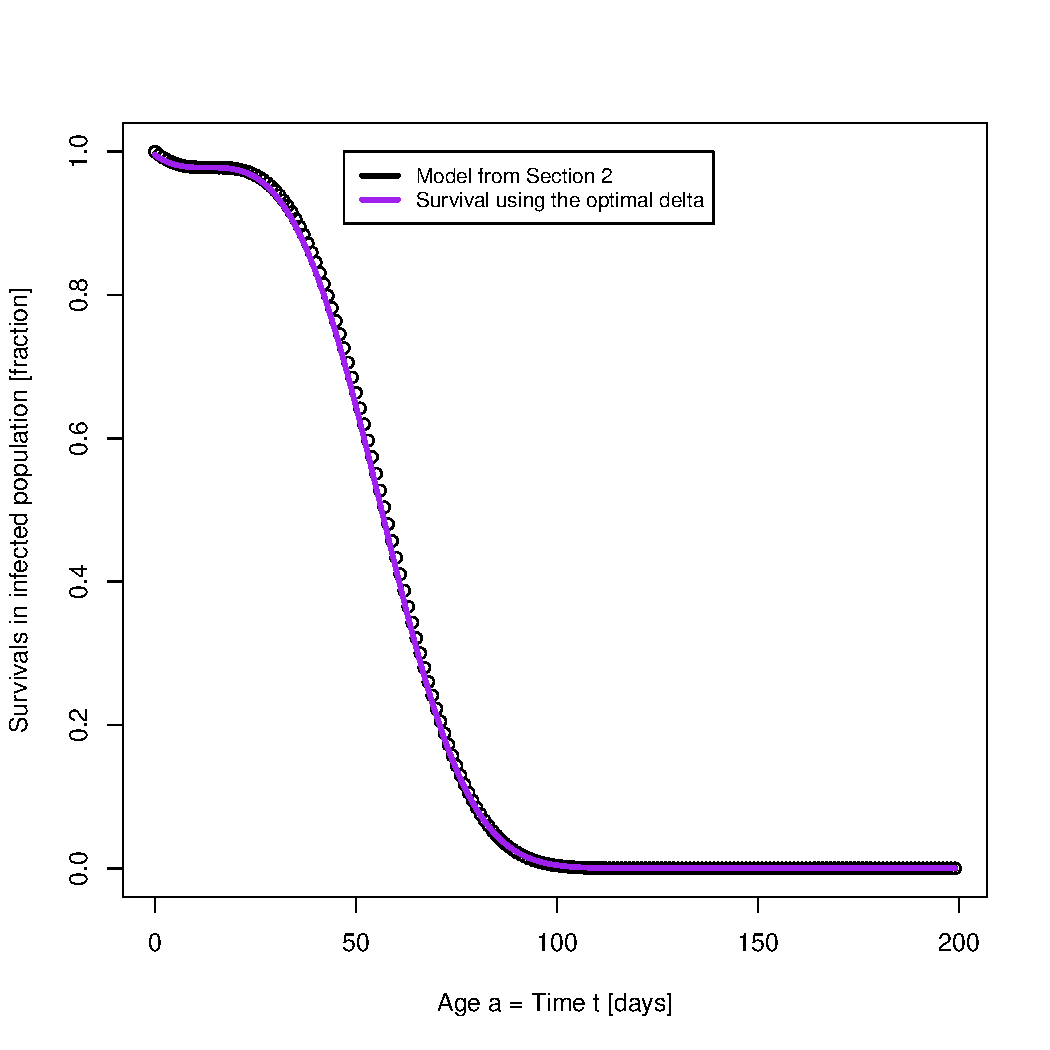
\includegraphics[width=\textwidth]{Comparison_of_models_infecteds.pdf}
    \caption{Comparison of the models for the infected population}
    \label{fig:subfigure_4}
  \end{subfigure}
\caption{Comparison of the plots obtained by the models from Section~\ref{rcode} and the plots obtained during the fitting of the delta to the data using MLE}
	\label{fig:comparison_survival_curve}
\end{figure}

In the Figure~\ref{fig:comparison_survival_curve} we can see that we achieved a good match when restricting our general model in Section~\ref{rcode} to the special case we used for the estimate of the death rates. This is not that much of a surprise, since those models are basically equivalent under the special case of non-interacting and non-reproducing populations. Only difference is, that the survivals plotted by the purple lines are computed throught the analytical expression for the survivals (the exponentials), so it should be in generally more precise than the dotted black plots.

From the above we can also trivially infere on the virulence, for the non-interacting populations which is just the difference:
\begin{equation}
v(a) = \delta^{inf}(a) - \delta^{inf}(a)
\end{equation}

\bibliographystyle{unsrtnat}
\bibliography{bibliography_SIE_model}

\end{document}

